\باب{چھلنی}


\حصہ{چھلنی}
اشارات کو تعدد کی بنیاد پر علیحدہ کرنے کے لئے \اصطلاح{چھلنی}\فرہنگ{چھلنی}\حاشیہب{filter}\فرہنگ{filter} استعمال کی جاتی ہے۔ان میں پست گزار، بلند گزار، پٹی گزار اور پٹی روک چھلنیاں نہایت مقبول ہیں جن کے خط شکل \حوالہ{شکل_تعددی_چھلنی_کے_اقسام} میں دکھائے گئے ہیں۔\اصطلاح{پست گزار چھلنی}\فرہنگ{پست گزار چھلنی}\فرہنگ{چھلنی!پست گزار}\حاشیہب{low-pass filter}\فرہنگ{low-pass filter}\فرہنگ{filter!low-pass} کسی مخصوص تعدد \عددی{\omega_0} سے کم تعدد کے اشارات کو گزرنے دیتی ہے جبکہ بقایا تعدد کے اشارات کو روکتی ہے۔\اصطلاح{بلند گزار چھلنی}\فرہنگ{بلند گزار چھلنی}\فرہنگ{چھلنی!بلند گزار}\حاشیہب{high-pass filter}\فرہنگ{high-pass filter}\فرہنگ{filter!high-pass} کسی مخصوص تعدد \عددی{\omega_0} سے زیادہ تعدد کے اشارات کو گزرنے دیتی ہے جبکہ بقایا تعدد کے اشارات کو روکتی ہے۔\اصطلاح{پٹی گزار چھلنی}\فرہنگ{پٹی گزار چھلنی}\فرہنگ{چھلنی!پٹی گزار}\حاشیہب{band-pass filter}\فرہنگ{band-pass filter}\فرہنگ{filter!band-pass} کسی مخصوص تعددی پٹی \عددی{\omega_L} تا \عددی{\omega_H} کے اشارات کو گزرنے دیتی ہے جبکہ بقایا تعدد کے اشارات کو روکتی ہے۔\اصطلاح{پٹی روک چھلنی}\فرہنگ{پٹی روک چھلنی}\فرہنگ{چھلنی!پٹی روک}\حاشیہب{band-stop filter}\فرہنگ{band-stop filter}\فرہنگ{filter!band-stop} کسی مخصوص تعددی پٹی \عددی{\omega_L} تا \عددی{\omega_H} کے اشارات کو روکتی ہے جبکہ بقایا تعدد کے اشارات کو گزرنے دیتی ہے۔
\begin{figure}
\centering
\begin{tikzpicture}
\draw(0,0)--++(1.5*\x,0)node[below]{$\omega$};
\draw(0,0)--++(0,\y)node[left]{$\bA_v$};
\draw(0,1)node[left]{$1$}--++(3/4*\x,0)--++(0,-1);
\draw(3/4*\x,0)node[below]{$\omega_0$};
\draw(\x,1.5)node[above]{\RL{کامل پست گزار چھلنی}};
%
\begin{scope}[xshift=-5cm]
\draw(0,0)--++(1.5*\x,0)node[below]{$\omega$};
\draw(0,0)--++(0,\y)node[left]{$\bA_v$};
\draw(0,1)node[left]{$1$};
\draw(3/4*\x,0)--++(0,1)--++(3/4*\x,0);
\draw(3/4*\x,0)node[below]{$\omega_0$};
\draw(\x,1.5)node[above]{\RL{کامل بلند گزار چھلنی}};
\end{scope}
%==================
\begin{scope}[yshift=-5cm]
\draw(0,0)--++(1.5*\x,0)node[below]{$\omega$};
\draw(0,0)--++(0,\y)node[left]{$\bA_v$};
\draw(0,1)node[left]{$1$};
\draw(\x/2,0)node[below]{$\omega_L$}--++(0,1)--++(1,0)--++(0,-1)node[below]{$\omega_H$};
\draw(\x,1.5)node[above]{\RL{کامل پٹی گزار چھلنی}};
\end{scope}
%
\begin{scope}[xshift=-5cm,yshift=-5cm]
\draw(0,0)--++(1.5*\x,0)node[below]{$\omega$};
\draw(0,0)--++(0,\y)node[left]{$\bA_v$};
\draw(0,1)node[left]{$1$};
\draw(0,1)--++(\x/2,0)--++(0,-1)node[below]{$\omega_L$}++(1,0)node[below]{$\omega_H$}--++(0,1)--++(1,0);
\draw(\x,1.5)node[above]{\RL{کامل پٹی روک چھلنی}};
\end{scope}
\end{tikzpicture}
\caption{کامل چھلنیوں کے خط۔}
\label{شکل_تعددی_چھلنی_کے_اقسام}
\end{figure}
%
\begin{figure}
\centering
\begin{subfigure}{0.33\textwidth}
\centering
\begin{tikzpicture}[american voltages]
\draw(0,0) to [american voltage source,l={$\hat{V}_d$}]++(0,\y) to [resistor,l={$R$}]++(\x,0) to [capacitor,l_={$C$},v^<={$\hat{V}_0$}]++(0,-\y) to [short] (0,0);
\end{tikzpicture}
\caption*{(الف) پست گزار چھلنی کا سادہ ترین دور۔}
\end{subfigure}%
\begin{subfigure}{0.66\textwidth}
\centering
\begin{tikzpicture}
\begin{semilogxaxis}[small,xlabel={$\omega$},ylabel={$\abs{\bA_v(j\omega)}$},ylabel style={rotate=-90},ytick={1,0.707},yticklabels={$\SI{0}{\deci\bel}$,$\SI{-3}{\deci\bel}$},xtick={0.1,1,10},xticklabels={$\frac{\omega_0}{10}$,$\omega_0$,$10\omega_0$}]
\addplot[mark=none,color=black] coordinates {(0.1,1)  (1,1) (1,0) (10,0)};
\addplot[mark=none,color=black,domain=0.1:10,samples=30]{1/sqrt(1+x^2)}node[pos=0.6,pin=45:{\RL{حقیقی}}]{};
\addplot[mark=none,color=black]coordinates{(1,0.3)}node[pin=125:{\RL{کامل}}]{};
\end{semilogxaxis}
\end{tikzpicture}
\caption*{(ب) کامل اور حقیقی پست گزار چھلنی کے خط۔}
\end{subfigure}
\caption{پست گزار چھلنی۔}
\label{شکل_تعدد_کامل_پست_گزار_خصلت}
\end{figure}

شکل \حوالہ{شکل_تعدد_کامل_پست_گزار_خصلت}-الف میں پست گزار چھلنی کا سادہ ترین دور دکھایا گیا ہے جس کی افزائش دباو \عددی{\bA_v=\tfrac{\hat{V}_0}{\hat{V}_d}}  درج ذیل ہے
\begin{align*}
\bA_v(j\omega)&=\frac{1}{1+j\omega RC}\\
&=\frac{1}{1+j\omega \tau}
\end{align*} 
جہاں \عددی{RC=\tau} \اصطلاح{وقتی مستقل}\فرہنگ{وقتی مستقل}\حاشیہب{time constant}\فرہنگ{time constant} کہلاتا ہے۔افزائش دباو کی \اصطلاح{مقداری خصلت}\فرہنگ{مقداری خصلت}\فرہنگ{خصلت!مقداری}\حاشیہب{magnitude characteristic}\فرہنگ{magnitude characteristic}  اور \اصطلاح{زاویائی خصلت}\فرہنگ{زاویائی خصلت}\حاشیہب{phase characteristic}\فرہنگ{phase characteristic} لکھتے ہیں۔
\begin{align*}
\abs{\bA_v(\omega)}&=\frac{1}{\sqrt{1+\omega^2 \tau^2}}\\
\phase{\bA_v(\omega)}&=-\tan^{-1} \omega \tau
\end{align*}
شکل \حوالہ{شکل_تعدد_کامل_پست_گزار_خصلت}-ب میں کامل پست گزار چھلنی اور شکل-الف کے حقیقی چھلنی کے خط دکھائے گئے ہیں۔ اگرچہ ہم چاہتے ہیں کہ پست گزار چھلنی کسی مخصوص تعدد \عددی{\omega_0} سے کم تعدد کو جوں کا توں گزارے اور اس سے بلند تعدد کو قطعاً نہیں گزارے، حقیقی ادوار ایسا کرنے سے قاصر ہوتے ہیں۔کامل پست گزار چھلنی \اصطلاح{انقطاعی تعدد}\فرہنگ{انقطاعی تعدد}\حاشیہب{cut-off frequency}\فرہنگ{cut-off frequency} \عددی{\omega_0} سے کم تعدد کو مکمل طور پر گزارتی ہے جبکہ اس سے زیادہ تعدد کو مکمل طور پر روکتی ہے۔حقیقی پست گزار چھلنی بھی یہی کچھ کرتی ہے البتہ انقطاعی تعدد کے قریبی تعدد پر اس کی کارکردگی کامل نہیں ہوتی۔جیسا شکل-ب میں دکھایا گیا ہے، انقطاعی تعدد \عددی{\omega_0} پر حقیقی پست گزار چھلنی کی افزائش دباو \عددی{\A_v} تین ڈیسی بیل کم ہوتی ہے۔جیسا آپ نے بوڈا خطوط میں پڑھا تھا، انقطاعی تعدد کی تعریف یہ ہے کہ اس پر اشارے کی طاقت نصف ہو جائے۔اشارے کا حیطہ \عددی{\tfrac{1}{\sqrt{2}}} گنا ہونے سے اس کی طاقت آدھی ہوتی ہے۔جیسا شکل-ب سے واضح ہے، انقطاعی تعدد سے دور تعدد پر حقیقی پست گزار چھلنی کی کارکردگی یقیناً قابل تعریف ہے۔انقطاعی تعدد سے دس گنا کم \عددی{\tfrac{\omega_0}{10}} یا دس گنا زیادہ \عددی{10\omega_0} تعدد پر اس کی کارکردگی تقریباً کامل چھلنی جیسے ہے۔

شکل \حوالہ{شکل_تعدد_کامل_پست_گزار_خصلت}-الف میں دئے پست گزار چھلنی کو اس طرح سمجھا جا سکتا ہے کہ کم تعدد پر برق گیر کی رکاوٹ زیادہ ہوتی ہے لہٰذا تقسیم دباو کے کلیے سے ظاہر ہے کہ برق گیر پر زیادہ دباو پایا جائے گا۔اس کے برعکس زیادہ تعدد پر برق گیر کی رکاوٹ کم ہوتی ہے لہٰذا تقسیم دباو کے کلیے کے تحت اس پر دباو گھٹ جائے گا۔انتہائی بلند تعدد پر برق گیر کی رکاوٹ انتہائی کم ہو گی اور اس پر دباو قابل نظر انداز ہو گا۔

شکل \حوالہ{شکل_تعدد_کامل_بلند_گزار_خصلت}-الف میں بلند گزار چھلنی کا سادہ ترین دور دکھایا گیا ہے جس کی تبادلی تفاعل لکھتے ہیں جہاں \عددی{RC=\tau} لکھا گیا ہے۔
\begin{align*}
\bA_v(j\omega)&=\frac{R}{R+\frac{1}{j\omega C}}\\
&=\frac{j\omega C}{1+j\omega RC}\\
&=\frac{j\omega \tau}{1+j\omega \tau}
\end{align*}
تبادلی تفاعل کی مقداری اور زاویائی تفاعل لکھتے ہیں۔
\begin{align}
\abs{\bA_v(\omega)}&=\frac{\omega \tau}{\sqrt{1+\omega^2 \tau^2}}\\
\phase{\bA_v(\omega)}=90^{-circ}-\tan^{-1}\omega \tau
\end{align}
شکل-ب میں تبادلی تفاعل کا مقداری خط دکھایا گیا ہے۔ساتھ ہی کامل بلند گزار چھلنی کا خط بھی دکھایا گیا ہے۔یہاں بھی حقیقی چھلنی کی افزائش دباو انقطاعی تعدد پر اشارے کی طاقت آدھی کرتی ہے۔


شکل \حوالہ{شکل_تعدد_کامل_بلند_گزار_خصلت}-الف میں دئے بلند گزار چھلنی کو اس طرح سمجھا جا سکتا ہے کہ صفر تعدد کے قریب برق گیر کی رکاوٹ انتہائی زیادہ ہو گی لہٰذا تقسیم دباو کے کلیے سے ظاہر ہے کہ مزاحمت پر  دباو انتہائی کم ہو گا۔اس کے برعکس انتہائی زیادہ  تعدد پر برق گیر کی رکاوٹ انتہائی کم ہو گی لہٰذا تقسیم دباو کے کلیے کے تحت پورا دباو مزاحمت پر پایا جائے گا۔

\begin{figure}
\centering
\begin{subfigure}{0.33\textwidth}
\centering
\begin{tikzpicture}[american voltages]
\draw(0,0) to [american voltage source,l={$\hat{V}_d$}]++(0,\y) to [capacitor,l={$C$}]++(\x,0) to [resistor,l_={$R$},v^<={$\hat{V}_0$}]++(0,-\y) to [short] (0,0);
\end{tikzpicture}
\caption*{(الف) بلند گزار چھلنی کا سادہ ترین دور۔}
\end{subfigure}%
\begin{subfigure}{0.66\textwidth}
\centering
\begin{tikzpicture}
\begin{semilogxaxis}[small,xlabel={$\omega$},ylabel={$\abs{\bA_v(j\omega)}$},ylabel style={rotate=-90},ytick={1,0.707},yticklabels={$\SI{0}{\deci\bel}$,$\SI{-3}{\deci\bel}$},xtick={0.1,1,10},xticklabels={$\frac{\omega_0}{10}$,$\omega_0$,$10\omega_0$}]
\addplot[mark=none,color=black] coordinates {(0.1,0) (1,0)  (1,1)  (10,1)};
\addplot[mark=none,color=black,domain=0.1:10,samples=30]{x/sqrt(1+x^2)}node[pos=0.2,pin=125:{\RL{حقیقی}}]{};
\addplot[mark=none,color=black]coordinates{(1,0.3)}node[pin=45:{\RL{کامل}}]{};
\end{semilogxaxis}
\end{tikzpicture}
\caption*{(ب) کامل اور حقیقی بلند گزار چھلنی کے خط۔}
\end{subfigure}
\caption{بلند گزار چھلنی۔}
\label{شکل_تعدد_کامل_بلند_گزار_خصلت}
\end{figure}

پٹی گزار چھلنی کا سادہ ترین دور شکل \حوالہ{شکل_تعدد_کامل_پٹی_گزار_خصلت} میں دکھایا گیا ہے۔اس کی افزائش دباو لکھتے ہوئے
\begin{gather}
\begin{aligned}\label{مساوات_تعددی_پٹی_گزار_دور_مساوات}
\bA_v(j\omega)&=\frac{R}{R+j\left(\omega L-\frac{1}{\omega C}\right)}\\
&=\frac{\omega RC}{\omega RC +j(\omega^2 LC-1)}
\end{aligned}
\end{gather}
مقداری تفاعل لکھتے ہیں
\begin{align}\label{مساوات_تعددی_پٹی_گزار_دور_حتمی}
\abs{\bA_v(\omega)}&=\frac{\omega RC}{\sqrt{(\omega RC)^2+(\omega^2 LC-1)^2}}
\end{align}
جس کو شکل-ب میں دکھایا گیا ہے۔اس کی کارکردگی یوں سمجھی جا سکتی ہے کہ درمیانی تعدد یعنی گمکی تعدد \عددی{\omega_0} پر \عددی{\omega L-\tfrac{1}{\omega C}=0} ہوتا ہے لہٰذا داخلی اشارہ جوں کا توں مزاحمت پر پہنچتا ہے۔گمکی تعدد سے بہت کم تعدد پر برق گیر کی رکاوٹ بہت بڑھ جاتی ہے  لہٰذا تقسیم دباو کے کلیے سے ظاہر ہے کہ مزاحمت پر دباو بہت کم ہو گی۔اسی طرح گمکی تعدد سے بہت زیادہ تعدد پر امالی رکاوٹ کی قیمت بہت بڑھ جاتی ہے جس کی وجہ سے مزاحمت پر دباو بہت کم ہوتی ہے۔
%
\begin{figure}
\centering
\begin{subfigure}{0.33\textwidth}
\centering
\begin{tikzpicture}[american voltages]
\draw(0,0) to [american voltage source,l={$\hat{V}_d$}]++(0,\y) to [inductor,l={$L$}]++(\x,0) to [capacitor,l={$C$}]++(\x,0) to [resistor,l_={$R$},v^<={$\hat{V}_0$}]++(0,-\y) to [short] (0,0);
\end{tikzpicture}
\caption*{(الف) پٹی گزار چھلنی کا سادہ ترین دور۔}
\end{subfigure}%
\begin{subfigure}{0.66\textwidth}
\centering
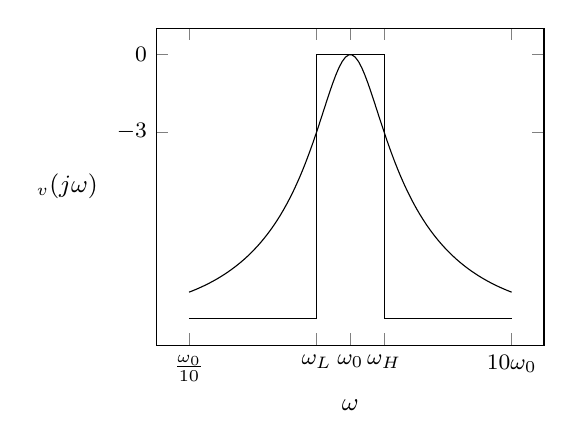
\begin{tikzpicture}
\begin{semilogxaxis}[small,xlabel={$\omega$},ylabel={$\abs{\bA_v(j\omega)}$},ylabel style={rotate=-90},ytick={1,0.707},yticklabels={$\SI{0}{\deci\bel}$,$\SI{-3}{\deci\bel}$},xtick={0.1,1,10,0.618,1.618},xticklabels={$\frac{\omega_0}{10}$,$\omega_0$,$10\omega_0$,$\omega_L$,$\omega_H$}]
\addplot[mark=none,color=black] coordinates {(0.1,0) (0.618,0)  (0.618,1) (1.618,1) (1.618,0) (10,0)};
\addplot[mark=none,color=black,domain=0.1:10,samples=100]{x/sqrt(x^2+(x^2-1)^2)};
\end{semilogxaxis}
\end{tikzpicture}
\caption*{(ب) کامل اور حقیقی پٹی گزار چھلنی کے خط۔}
\end{subfigure}
\caption{پٹی گزار چھلنی۔}
\label{شکل_تعدد_کامل_پٹی_گزار_خصلت}
\end{figure}

مساوات \حوالہ{مساوات_تعددی_پٹی_گزار_دور_مساوات} میں صرف \عددی{\omega} متغیر مقدار ہے۔افزائش دباو کی زیادہ سے زیادہ قیمت  اس تعدد \عددی{\omega_0} پر حاصل ہو گی جس پر نسب نما میں قوسین کی قیمت صفر کے برابر ہو یعنی
\begin{align}
\omega_0=\frac{1}{\sqrt{LC}}
\end{align} 
اس تعدد پر \عددی{\abs{\bA_v(\omega_0)}=\SI{1}{\volt\per\volt}} حاصل ہوتا ہے۔انقطاعی تعدد پر افزائش دباو \عددی{\abs{\bA_v(\omega_0)}} کے \عددی{\tfrac{1}{\sqrt{2}}} گنا ہو گی۔یوں مساوات \حوالہ{مساوات_تعددی_پٹی_گزار_دور_حتمی} کو استعمال کرتے ہوئے انقطاعی تعدد کے لئے درج ذیل لکھا جا سکتا ہے۔
\begin{align*}
\frac{\omega RC}{\sqrt{(\omega RC)^2+(\omega^2 LC-1)^2}}=\frac{1}{\sqrt{2}}
\end{align*}
دونوں جانب مربع لیتے اور ترتیب دیتے ہوئے درج ذیل
\begin{align*}
(\omega^2 LC-1)^2=(\omega RC)^2
\end{align*}
یعنی
\begin{align*}
\omega^2 LC-1=\mp \omega RC
\end{align*}
یا
\begin{align*}
\omega^2 LC\pm \omega RC-1=0
\end{align*}
ملتا ہے۔اس دو درجی مساوات کے حل لکھتے ہیں
\begin{align}
\omega_L&=\frac{-\frac{R}{L}+\sqrt{\left(\frac{R}{L}\right)^2+\frac{1}{LC}}}{2}\\
\omega_H&=\frac{+\frac{R}{L}+\sqrt{\left(\frac{R}{L}\right)^2+\frac{1}{LC}}}{2}
\end{align}
جن سے پٹی گزار چھلنی کی عرض پٹی \عددی{\BW} حاصل ہوتی ہے۔
\begin{align}
\BW=\omega_H-\omega_L=\frac{R}{L}
\end{align}
%===================
\ابتدا{مثال}
اگر آپ کو حساس اشارات کے ساتھ کام کرنا پڑے تو آپ دیکھیں گے کہ ان میں واپڈا کا \عددی{\SI{50}{\hertz}} پایا جاتا ہے جس سے چھٹکارا حاصل کرنا نہایت مشکل ہوتا ہے۔موبائل ٹیلیفون کے زمانے سے پہلے زمینی تار والے ٹیلیفون استعمال کئے جاتے تھے جن کی تاروں میں عموماً \عددی{\SI{50}{\hertz}} کا غیر مطلوب اشارہ گھس جاتا تھا جو شہد کی مکھی کی طرح ہوں ہوں کرتا سنائی دیتا تھا۔

میری بیٹی عفت بریخنہ نے انجنیئرنگ کے آخری سال میں \اصطلاح{برقی قلب نگار}\فرہنگ{برقی قلب نگار}\حاشیہب{electrocardiogram, ecg}\فرہنگ{electrocardiogram}\فرہنگ{ecg} بنایا۔انہیں مسلسل \عددی{\SI{50}{\hertz}} کے غیر مطلوب اشارے کا سامنہ کرنا پڑا۔پچاس ہرٹز کے غیر مطلوب اشارے کی خاصیت یہ ہے کہ اس کی تعدد اٹل ہے۔اس سے \اصطلاح{دندانہ چھلنی}\فرہنگ{دندانہ چھلنی}\فرہنگ{چھلنی!دندانہ}\حاشیہب{notch filter}\فرہنگ{notch filter}\فرہنگ{filter!notch} کی مدد سے چھٹکارا حاصل کیا جاتا ہے۔شکل میں دندانہ چھلنی کا دور دکھایا گیا ہے۔تار کے ٹیلیفون میں \عددی{R} سپیکر کی مزاحمت ہو گی۔برقی قلب نگار میں \عددی{R} اگلے دور کا داخلی تھونن مزاحمت ہو گا۔
\begin{figure}
\centering
\begin{tikzpicture}
\draw(0,0) to [short,o-]++(\x/2,0) to [capacitor,l={$C$}]++(\x,0) to [short,-o]++(\x,0);
\draw(0,-\y) to [short,o-o]++(2*\x+\x/2,0);
\draw(2*\x,0) to [resistor,*-*,l_={$R$}]++(0,-\y);
\draw(\x/2,0) to [short,*-]++(0,-\y/2)to[inductor,l_={$L$}] ++(\x,0) to [short,-*]++(0,\y/2);
\draw(0,-\y/2)node{$\begin{aligned} &+ \\ &\hat{V}_d \\ &- \end{aligned}$};
\draw(2*\x+\x/2,-\y/2)node{$\begin{aligned} &+ \\ &\hat{V}_0 \\ &- \end{aligned}$};
\end{tikzpicture}
\caption{دندانہ چھلنی کی مدد سے \عددی{\SI{50}{\hertz}} سے چھٹکارا حاصل کیا جاتا ہے۔}
\label{شکل_تعددی_دندانہ_چھلنی}
\end{figure}

متوازی امالہ گیر اور برق گیر کی رکاوٹ \عددی{\bZ} لکھتے ہیں۔
\begin{align*}
\bZ&=\frac{(j\omega L)(\frac{1}{j\omega C})}{j\omega L+\frac{1}{j\omega C}}\\
&=\frac{\frac{L}{C}}{j\omega L+ \frac{1}{j\omega C}}
\end{align*}
تقسیم دباو کے کلیے سے خارجی دباو لکھتے ہیں
\begin{align*}
\hat{V}_0&=\left(\frac{R}{R+Z}\right)\hat{V}_d\\
&=\frac{R \hat{V}_d}{R+\frac{\frac{L}{C}}{j\omega L+ \frac{1}{j\omega C}}}
\end{align*}
جس سے درج ذیل تبادلی تفاعل حاصل ہوتا ہے۔
\begin{align*}
\frac{\hat{V}_0}{\hat{V}_d}=\frac{(j\omega)^2+\frac{1}{LC}}{(j\omega)^2+\left(\frac{j\omega}{RC}\right)+\frac{1}{LC}}
\end{align*}
غیر مطلوب اشارے سے چھٹکارے کے لئے ضروری ہے کہ \عددی{\SI{50}{\hertz}} یعنی \عددی{100\pi\,\si{\radian\per\second}} پر تبادلی تفاعل  صفر کے برابر ہو۔یوں تبادلی تفاعل کا شمار کنندہ اس تعدد پر صفر کے برابر درکار ہے جس سے درج ذیل شرط حاصل ہوتی ہے۔
\begin{align}
\omega_0=\frac{1}{\sqrt{LC}}=100\pi
\end{align}
یوں برق گیر کی قیمت \عددی{\SI{100}{\micro\farad}} چنتے ہوئے امالہ کی قیمت \عددی{\SI{101.3}{\milli\henry}} حاصل ہوتی ہے۔دندانہ چھلنی کی کارکردگی دیکھنے کی خاطر داخلی اشارے \عددی{v_d(t)} کو \عددی{\SI{50}{\hertz}} اور \عددی{\SI{1000}{\hertz}} کے سائن نما اشارات کا مجموعہ تصور کرتے ہیں جہاں 
\begin{align*}
v_d(t)=1\cos (2\pi 50 t)+0.1\cos(2\pi 1000 t)
\end{align*}
شکل میں داخلی اور خارجی اشارات دکھائے گئے ہیں۔آپ دیکھ سکتے ہیں کہ \عددی{\SI{50}{\hertz}} سے مکمل چھٹکارا حاصل ہوا ہے۔ 
\انتہا{مثال}
%==================================
